\documentclass[pdf,15pt]{beamer}
\mode<presentation>{\usetheme{Warsaw}}
\usepackage{fontspec}   %加這個就可以設定字體
\usepackage{xeCJK}       %讓中英文字體分開設置

%
\usepackage{graphicx} % Allows including images
\usepackage{booktabs} % Allows the use of \toprule, \midrule and \bottomrule in tables
\setCJKmainfont{微軟正黑體} %設定中文為系統上的字型,而英文不去更動,使用原TeX字型
\XeTeXlinebreaklocale "zh"             %這兩行一定要加,中文才能自動換行
\XeTeXlinebreakskip = 0pt plus 1pt     %這兩行一定要加,中文才能自動換行

%% preamble
\title{C/C++基礎程式設計班}
\subtitle{C/C++程式語言簡介}
\author{曹又霖}

\defbeamertemplate{footline}{centered page number}
{%
  \hspace*{\fill}%
  \usebeamercolor[fg]{page number in head/foot}%
  \usebeamerfont{page number in head/foot}%
  \insertpagenumber\,/\,\insertpresentationendpage%
  \hspace*{\fill}\vskip2pt%
}

\setbeamertemplate{footline}[centered page number]
\setbeamertemplate{caption}[numbered]

\begin{document}

%% title frame
\begin{frame}
	\titlepage
\end{frame}

\begin{frame}
\frametitle{大綱} % Table of contents slide, comment this block out to remove it
\tableofcontents % Throughout your presentation, if you choose to use \section{} and \subsection{} commands, these will automatically be printed on this slide as an overview of your presentation
\end{frame}

\begin{section}{編譯器}
%% normal frame
\begin{subsection}{程式語言}
\begin{frame}{程式語言}
	\begin{itemize}
	\item 機器語言(Machine Language)
		\begin{itemize}
		\item 電腦使用0與1所組成的語言。
		\end{itemize}
	\item 高階程式語言
		\begin{itemize}
		\item 人比較可以看的懂的語言,用英文與數學符號所構成。
		\item 很好轉換成機器語言,藉此成為人與電腦溝通的橋梁。
		\end{itemize}
	\end{itemize}
	\begin{figure}[h!]
		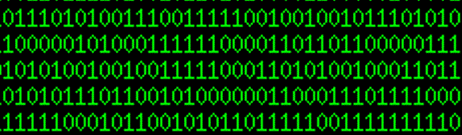
\includegraphics[width=0.5\textwidth]{image/00-01.png} 
		\caption{機器語言}
	\end{figure}
\end{frame}
\end{subsection}

\begin{subsection}{編譯器}
\begin{frame}{編譯器(Compiler)}
	\begin{itemize}
		\item 透過編譯器可以將人看的懂的程式語言轉換成電腦看的懂的機器語言。
		\item 這個動作就稱為「編譯(Compile)」。
	\end{itemize}
	
\end{frame}
\end{subsection}


\end{section}

\end{document}
